\documentclass[onecolumn]{article}
\usepackage{graphicx} % Required for inserting images
\usepackage{amsmath}
\usepackage{amsfonts}
\usepackage{pythonhighlight}
\usepackage{datetime}
\usepackage[colorlinks]{hyperref}
\usepackage{titling}
\usepackage{matlab-prettifier}
\usepackage[a4paper, total={6in, 8in}]{geometry}

\makeatletter
\Hy@AtBeginDocument{%
  \def\@pdfborder{0 0 1}% Overrides border definition set with colorlinks=true
  \def\@pdfborderstyle{/S/U/W 1}% Overrides border style set with colorlinks=true
                                % Hyperlink border style will be underline of width 1pt
}
\makeatother

\hypersetup{%
  colorlinks=true,
  linkcolor=blue,
  linkbordercolor=blue,% 
}
\footskip = 1pt
\textheight = 700pt
\setlength{\droptitle}{-10em}

\title{Lab 2 Extra \\ \Large{IN3170 - Microelectronics}}
\author{Andreas Engøy, Erik Røset \& Daniel Tran}
\date{\monthname[\the\month] \the\year}

\begin{document}
\maketitle
\vspace*{50mm}
\tableofcontents

\section{Task 1}

\subsection{Objective}
The objective of this task is to build two CMOS inverter chains of different length and probing before the first and after the last inverter. The purpose of this is to measure and calculate the propagation delay a single inverter without knowing the added capacitance of the scope probe or directly measuring the delay of just one inverter.

\subsection{Theory}

\begin{figure}[h!]
    \centering
    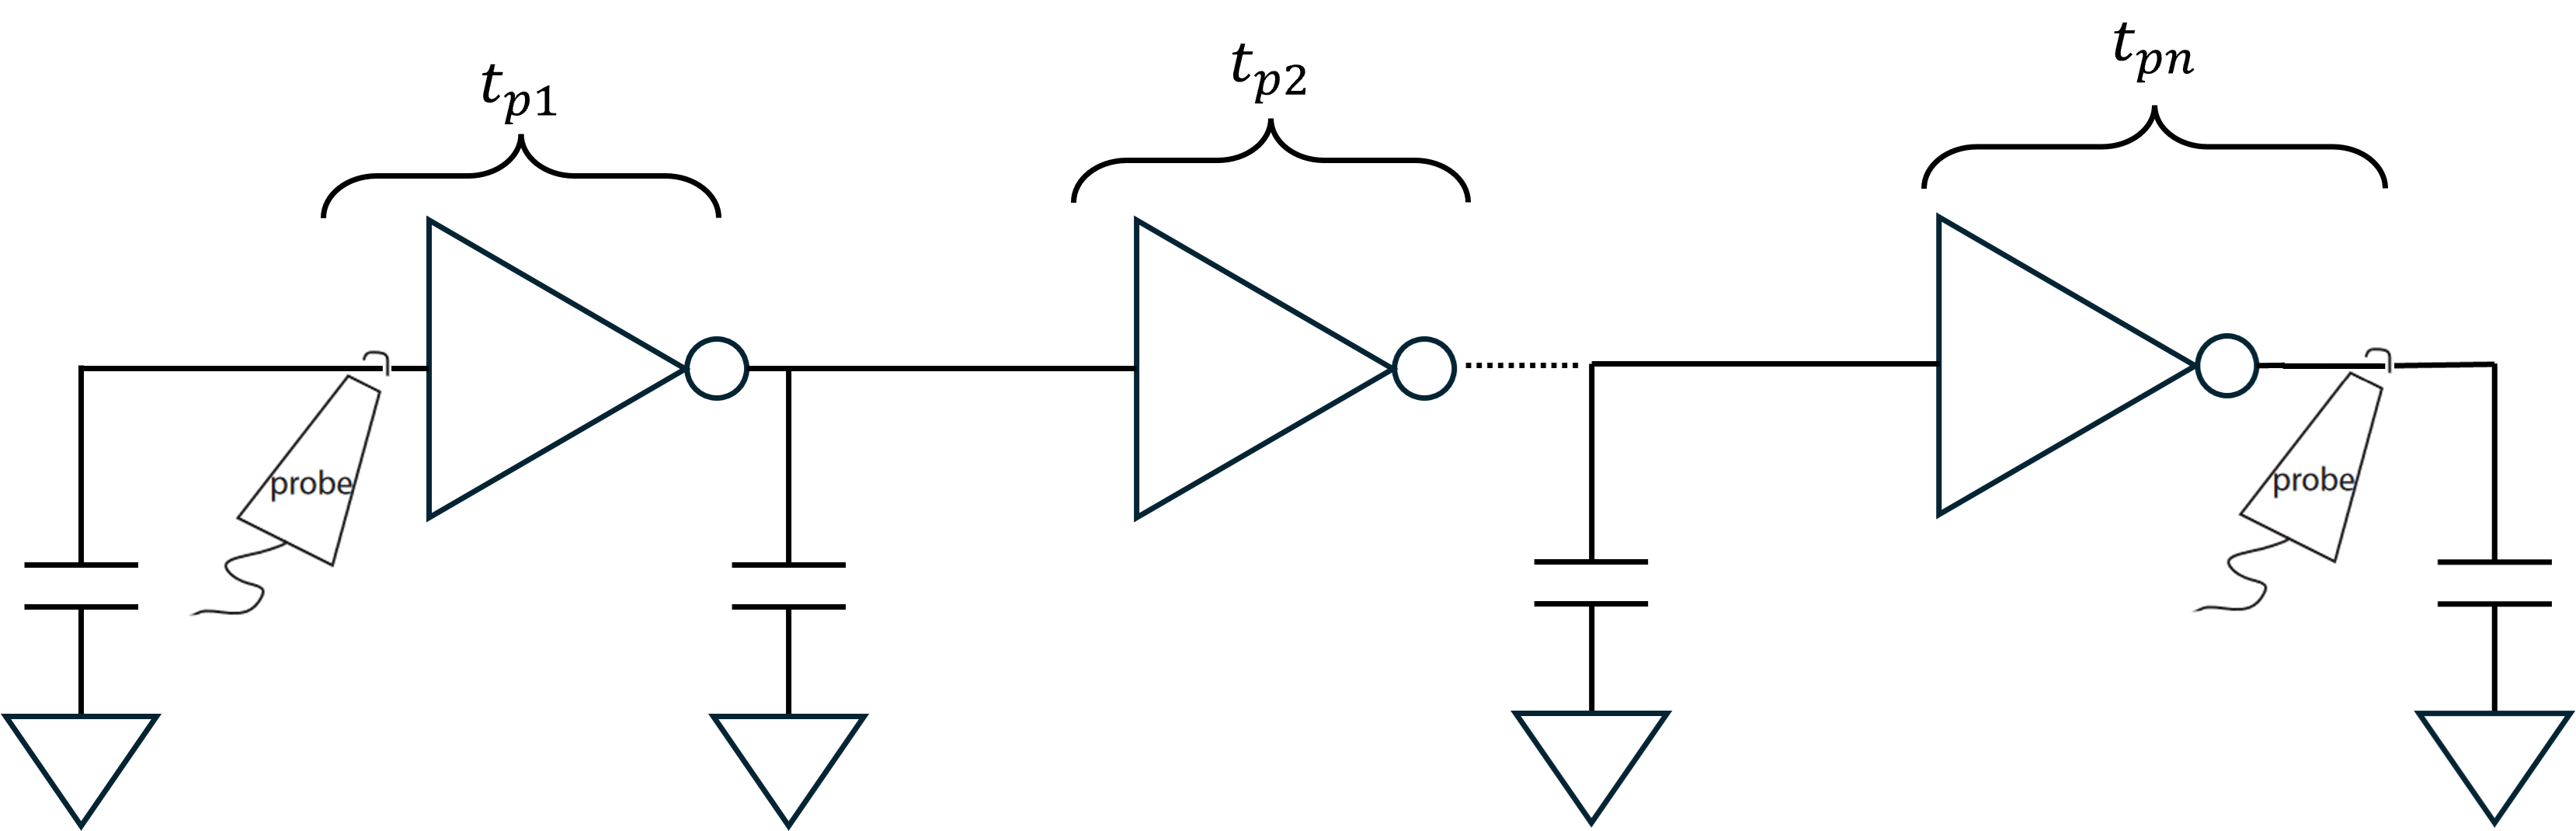
\includegraphics[width=0.75\textwidth]{illustration.png}
    \caption{Illustration of the different propegation delays for a inverter chain.}
    \label{fig:illustration}
\end{figure}

The total propagation delay of a chain of inverters is the sum of the propagation delay of each inverter. The oscilloscope probes used to measure the input and output signals add capacitance to the circuit, which can affect the measurement of the propagation delay. By measuring at the start and end of a inverter chain the added delay from the parasitic capacitance of the probes can be merged with the propagation delay of the first and last inverter as shown in figure \ref{fig:illustration}. I.e. the total propagation delay of a chain of inverters can be written as: 
\begin{equation}
    t_{p\_tot} = t_{p1} + t_{p2} + \cdots + t_{pn} 
\end{equation}

Where $t_{p1}$ and $t_{pn}$ also include the propagation delay introduced by the probes.

By then measuring the propagation delay of a chain of inverters with $n$ inverters and subtracting the propagation delay of a chain of inverters with $n-1$ inverters, the difference between the two would be the propagation delay of a single inverter without the added delay from the probes. This can be written as:

\begin{equation}
    t_{1inv} = t_{p\_tot(n)} - t_{p\_tot(n-1)} \label{eq:1inv}
\end{equation}

\subsection{Equipment}
\begin{table}[h!]
    \centering
    \begin{tabular}{|c|c|c|}
        \hline
        \textbf{Component} & \textbf{Model} & \textbf{Quantity} \\
        \hline
        Hex Scmitt-Trigger Inverters & SN74HC1 & 1 \\
        Oscilloscope & HP54622 & 1 \\
        Waveform generator  & HP33120 & 1\\
        Voltage source & HPE3631 & 1 \\
        Breadboard & $\sim$ & 1 \\
        \hline
    \end{tabular}
    \caption{List of components used in task 1.}
    \label{tab:bom}
\end{table}

\subsection{Method}

\begin{figure}[h!]
    \centering
    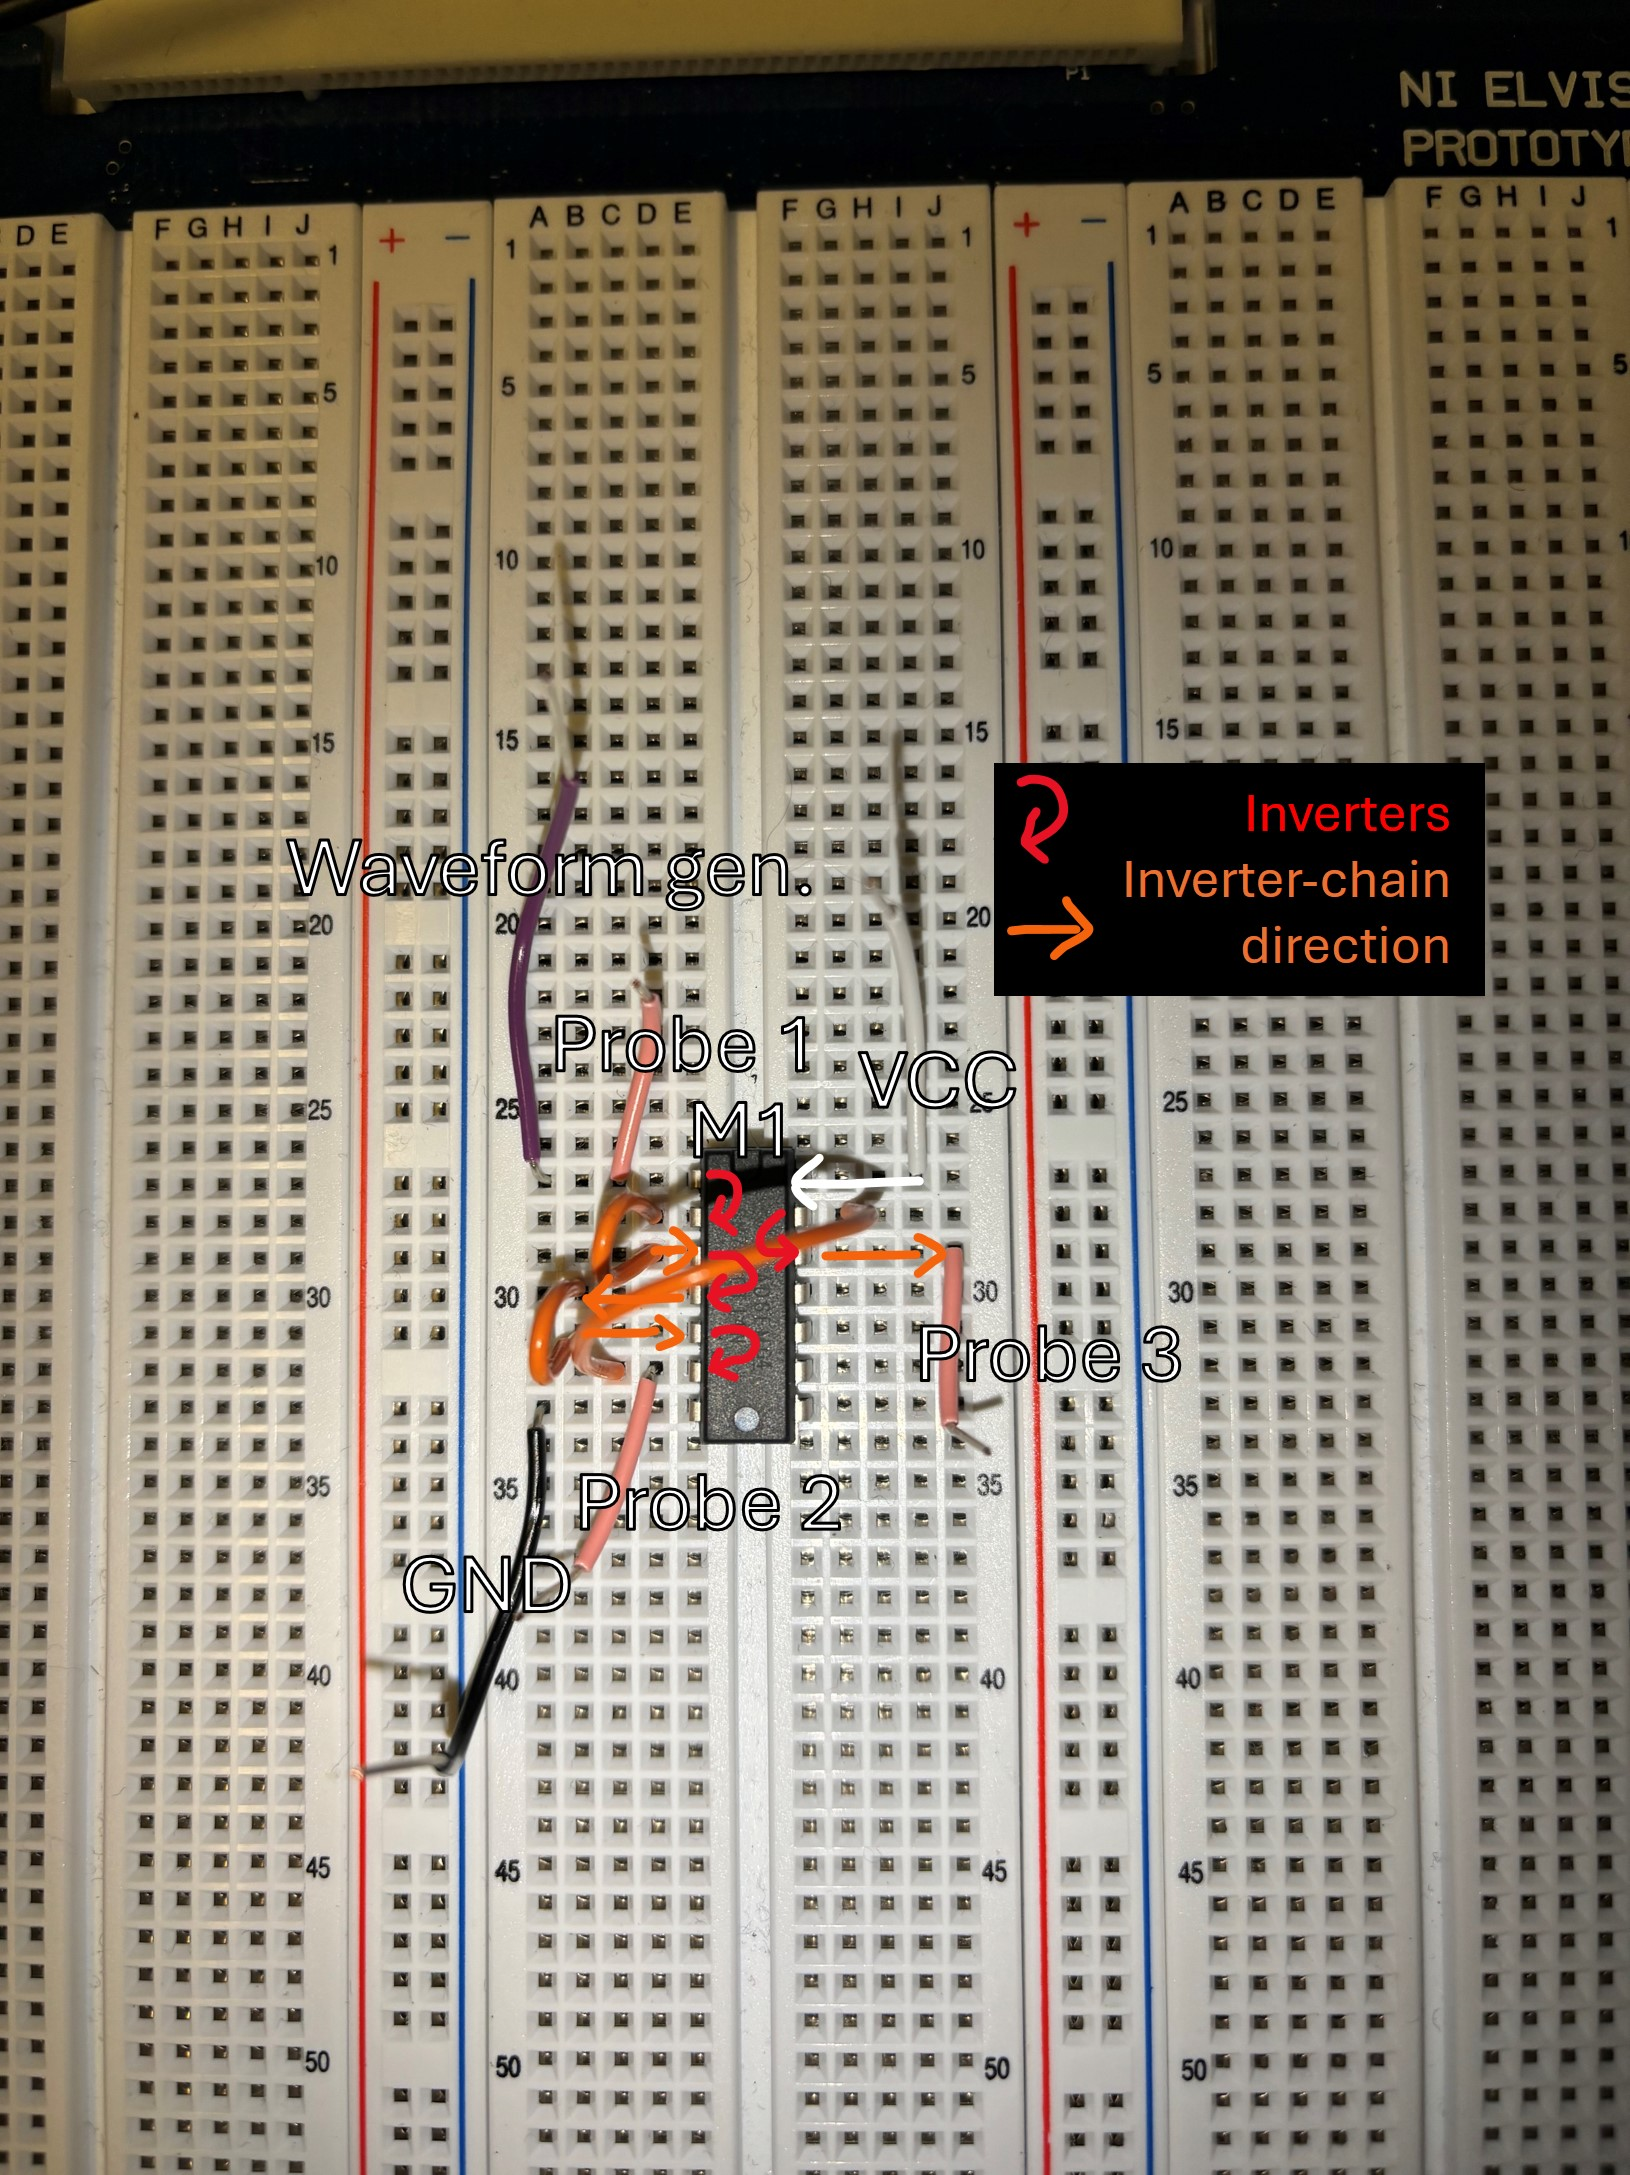
\includegraphics[width=0.5\textwidth]{Circuit_draw.jpg}
    \caption{Picture of the setup for task 1.}  
    \label{fig:circuit}
\end{figure}

\begin{figure}[h!]
    \centering
    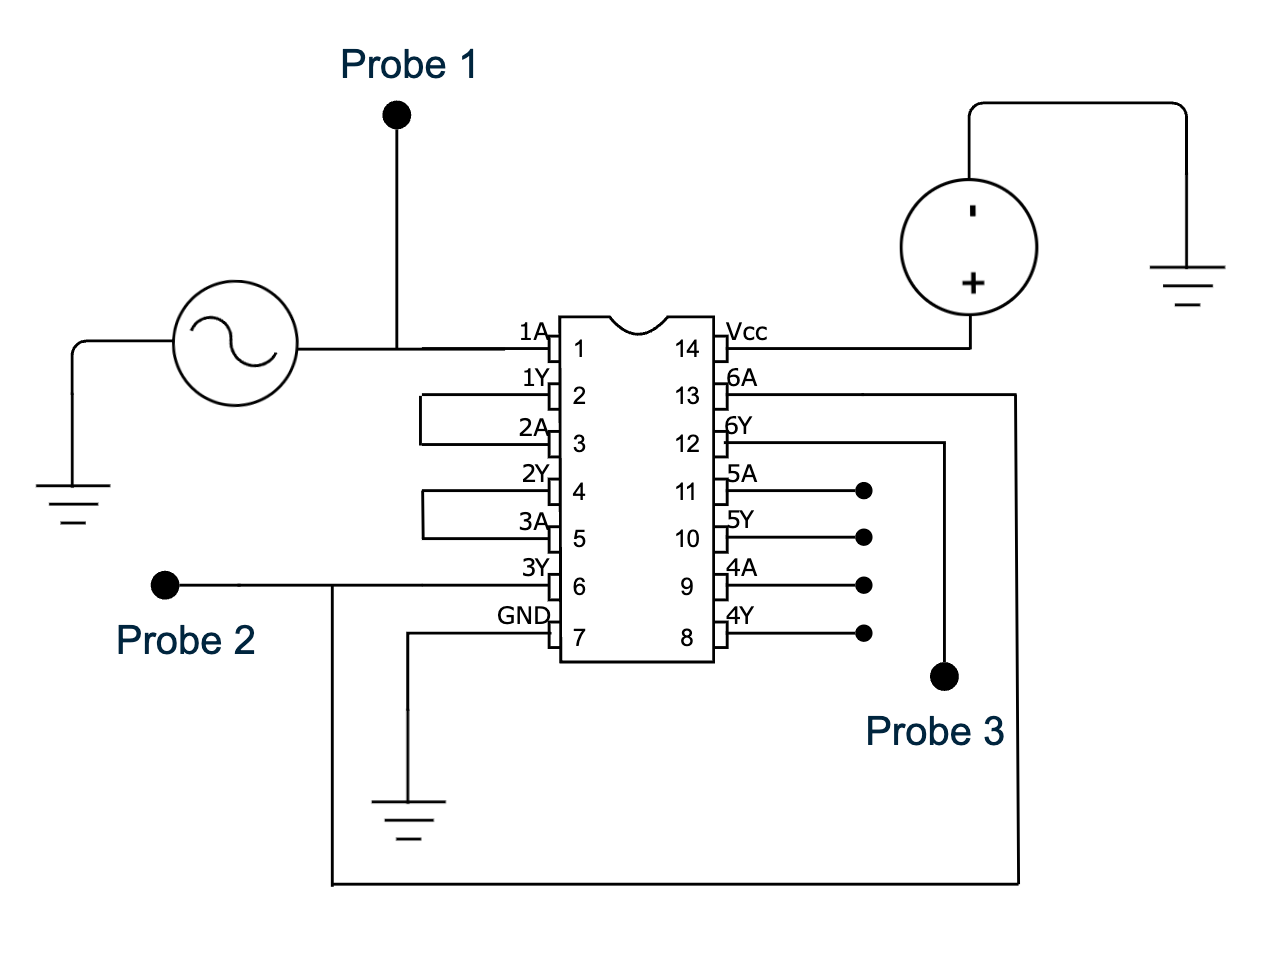
\includegraphics[width=0.5\textwidth]{circuit_schematics.png}
    \caption{Schematic of the setup for task 1.}
    \label{fig:schematic}
\end{figure}

On a breadboard, using $M1$ (SN74HC1) we built two inverter chains, one with 3 inverters and one with 4 inverters. At pin 1 a square wave with a frequency of 400 Hz, $V_{pp}$ of 2.1 V and $V_{off}$ of 1.1 V was connected. At pin 14 a 5 V power supply was connected. Pin 7 was connected to ground. In figure \ref{fig:circuit} and \ref{fig:schematic}; probe 1 is used to measure the input signal, probe 2 is used to measure the output after the third inverter and probe 3 is used to measure the output after the fourth inverter.

On the oscilloscope, channel 1 is connected to probe 1 and channel 2 is connected to probe 2 and 3, depending on if measuring for three or four inverters respectively. To reduce noise on the output, the built-in averaging filter of the oscilloscope was used. The X- and Y-axis were scaled to show one rising/falling edge of the input and output.

\clearpage

\subsection{Results}

\begin{figure}[h!]
    \centering
    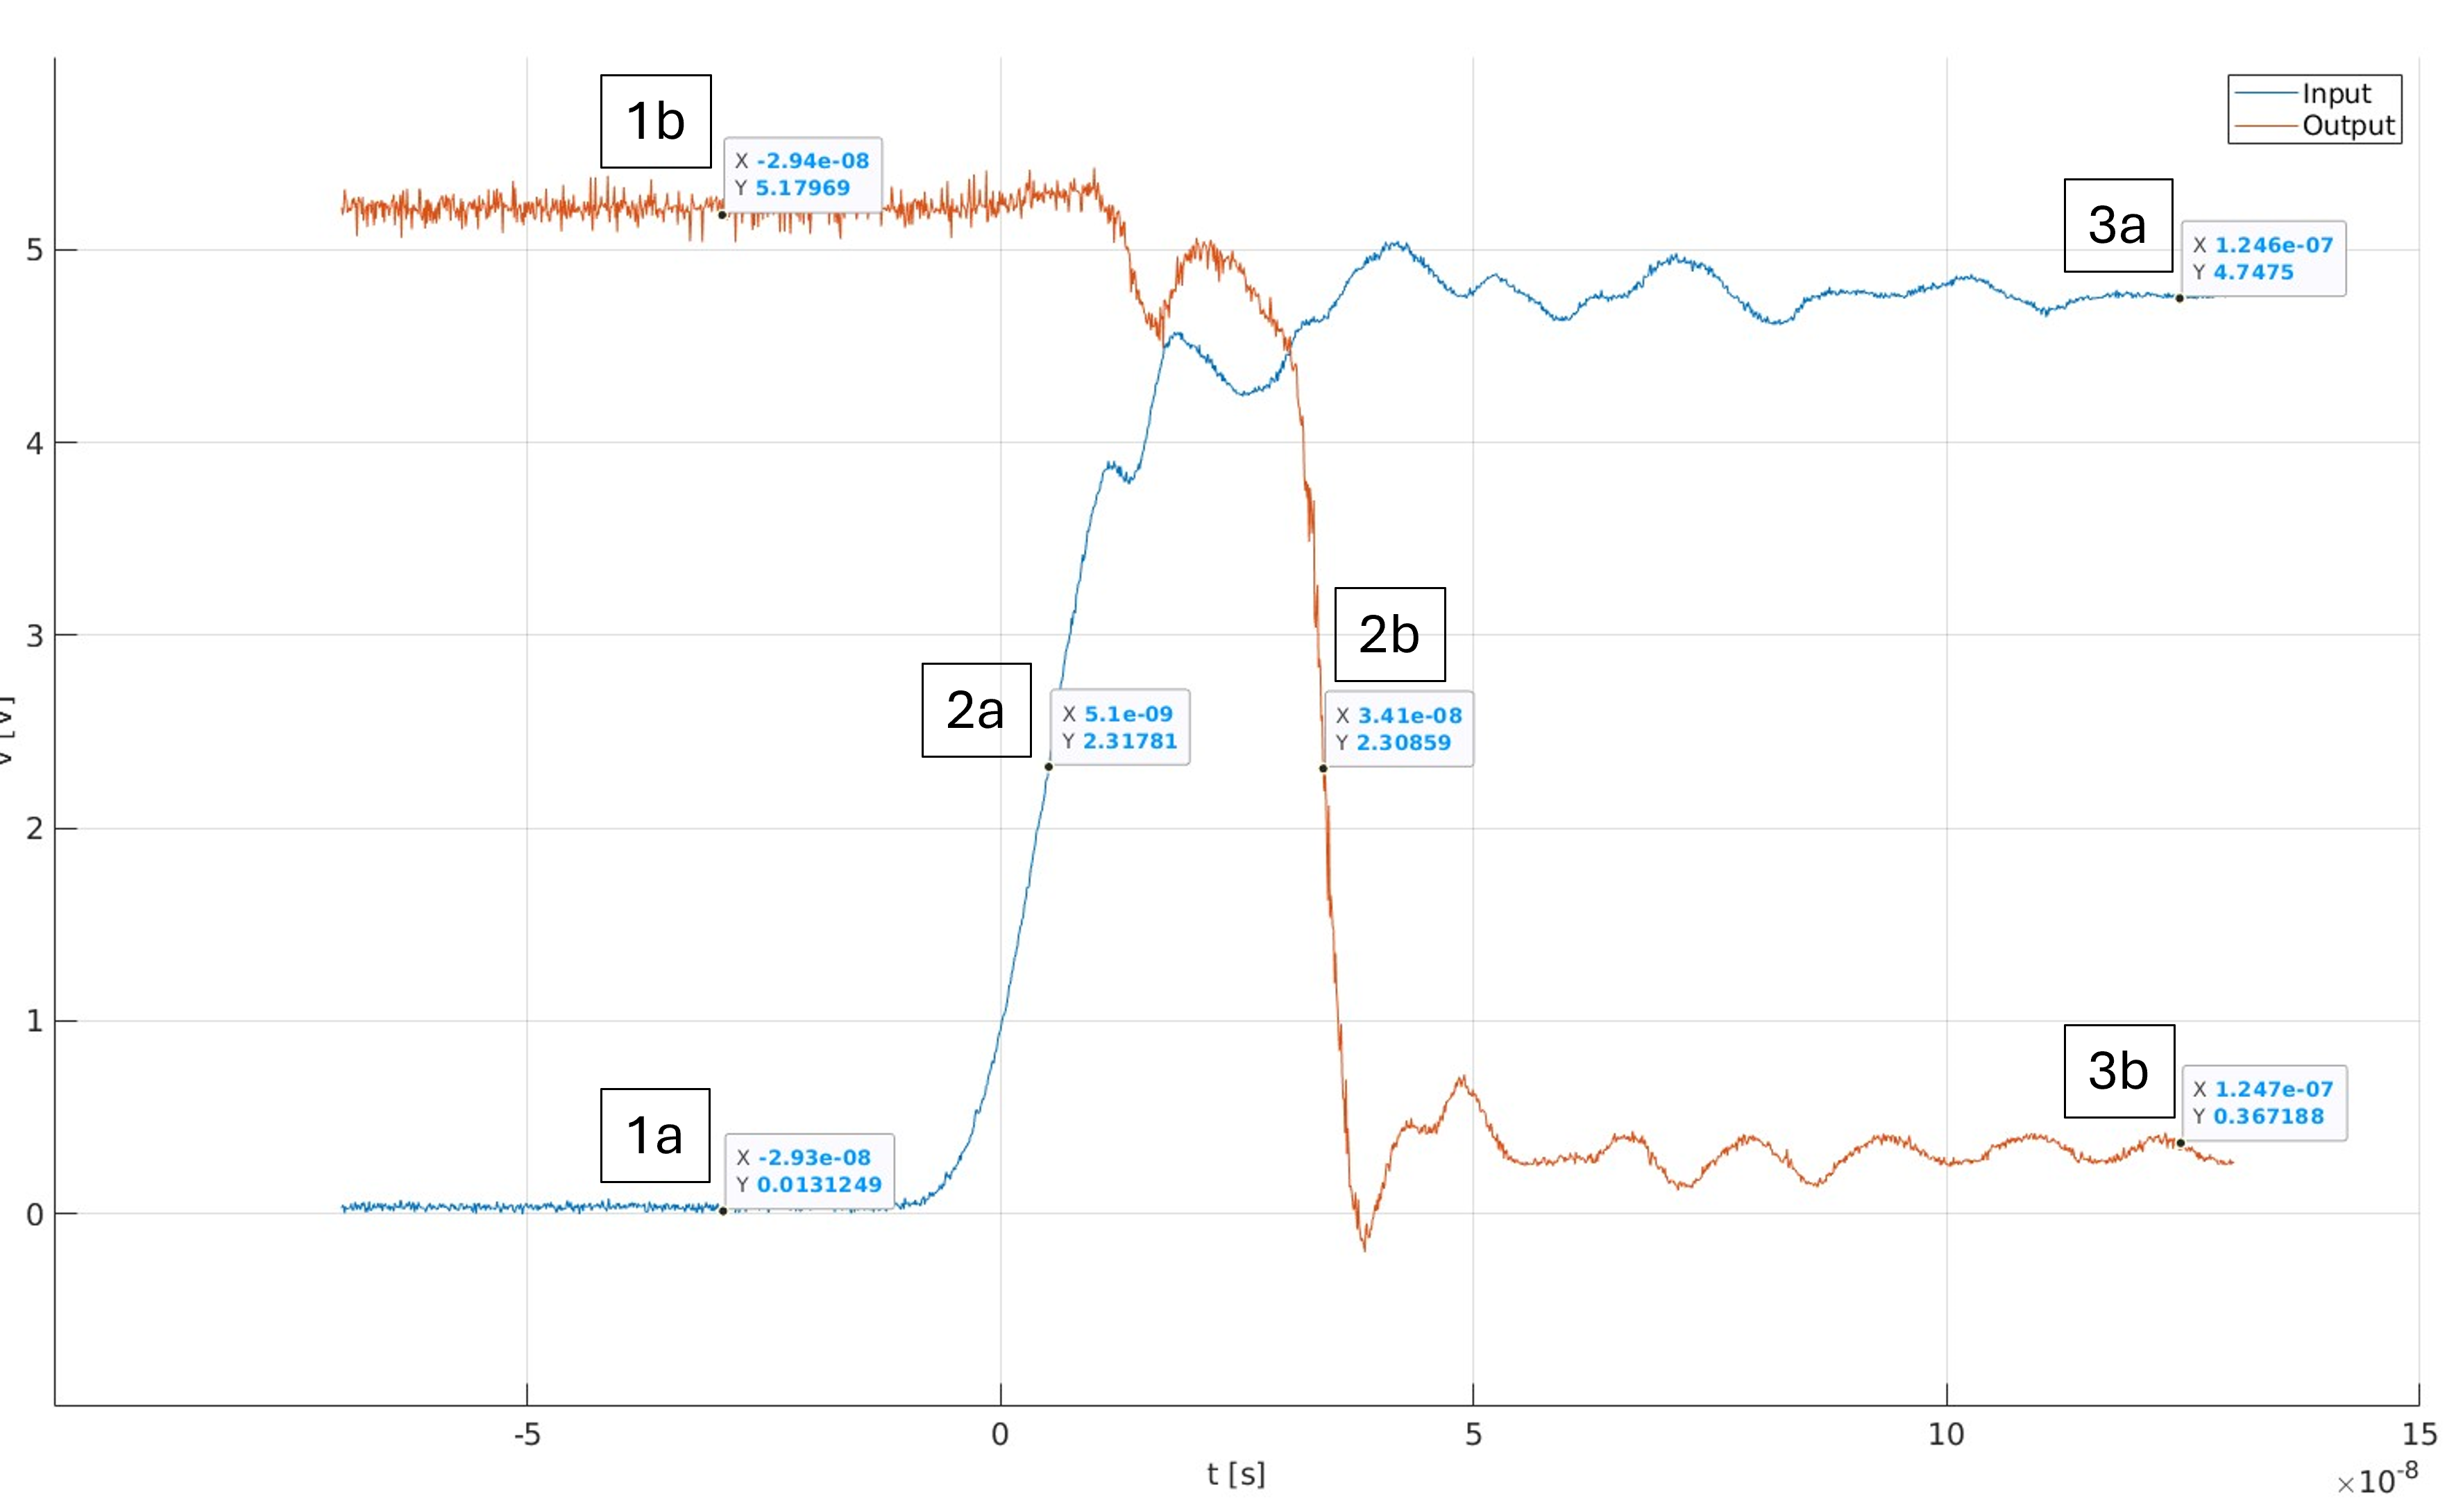
\includegraphics[width=0.75\textwidth]{3_inverters_marked.png}
    \caption{Rising edge of the input and falling edge of the output for the three inverter chain, with labeled marked points on the plot.}
    \label{fig:3inv}
\end{figure}

In figure \ref{fig:3inv} point 2a is used as the switching point for the input signal, somewhere around 50 \% of the rising edge. This point is estimated using point 1a as the low-signal and point 3a as the high-signal of the input signal. The same is done for the output signal in figure \ref{fig:3inv} using the points marked with 'b' instead.

The total propagation delay for the three inverter-chain is calculated as follows:
\begin{align}
    t_{in} &= 5.1\mathrm{e}{-9} \ \text{s} \\
    t_{out} &= 3.41\mathrm{e}{-8} \ \text{s} \\
    t_{3inv} &= t_{out} - t_{in} = 2.9\mathrm{e}{-8} \ \text{s} \label{eq:3inv}
\end{align}

\begin{figure}[h!]
    \centering
    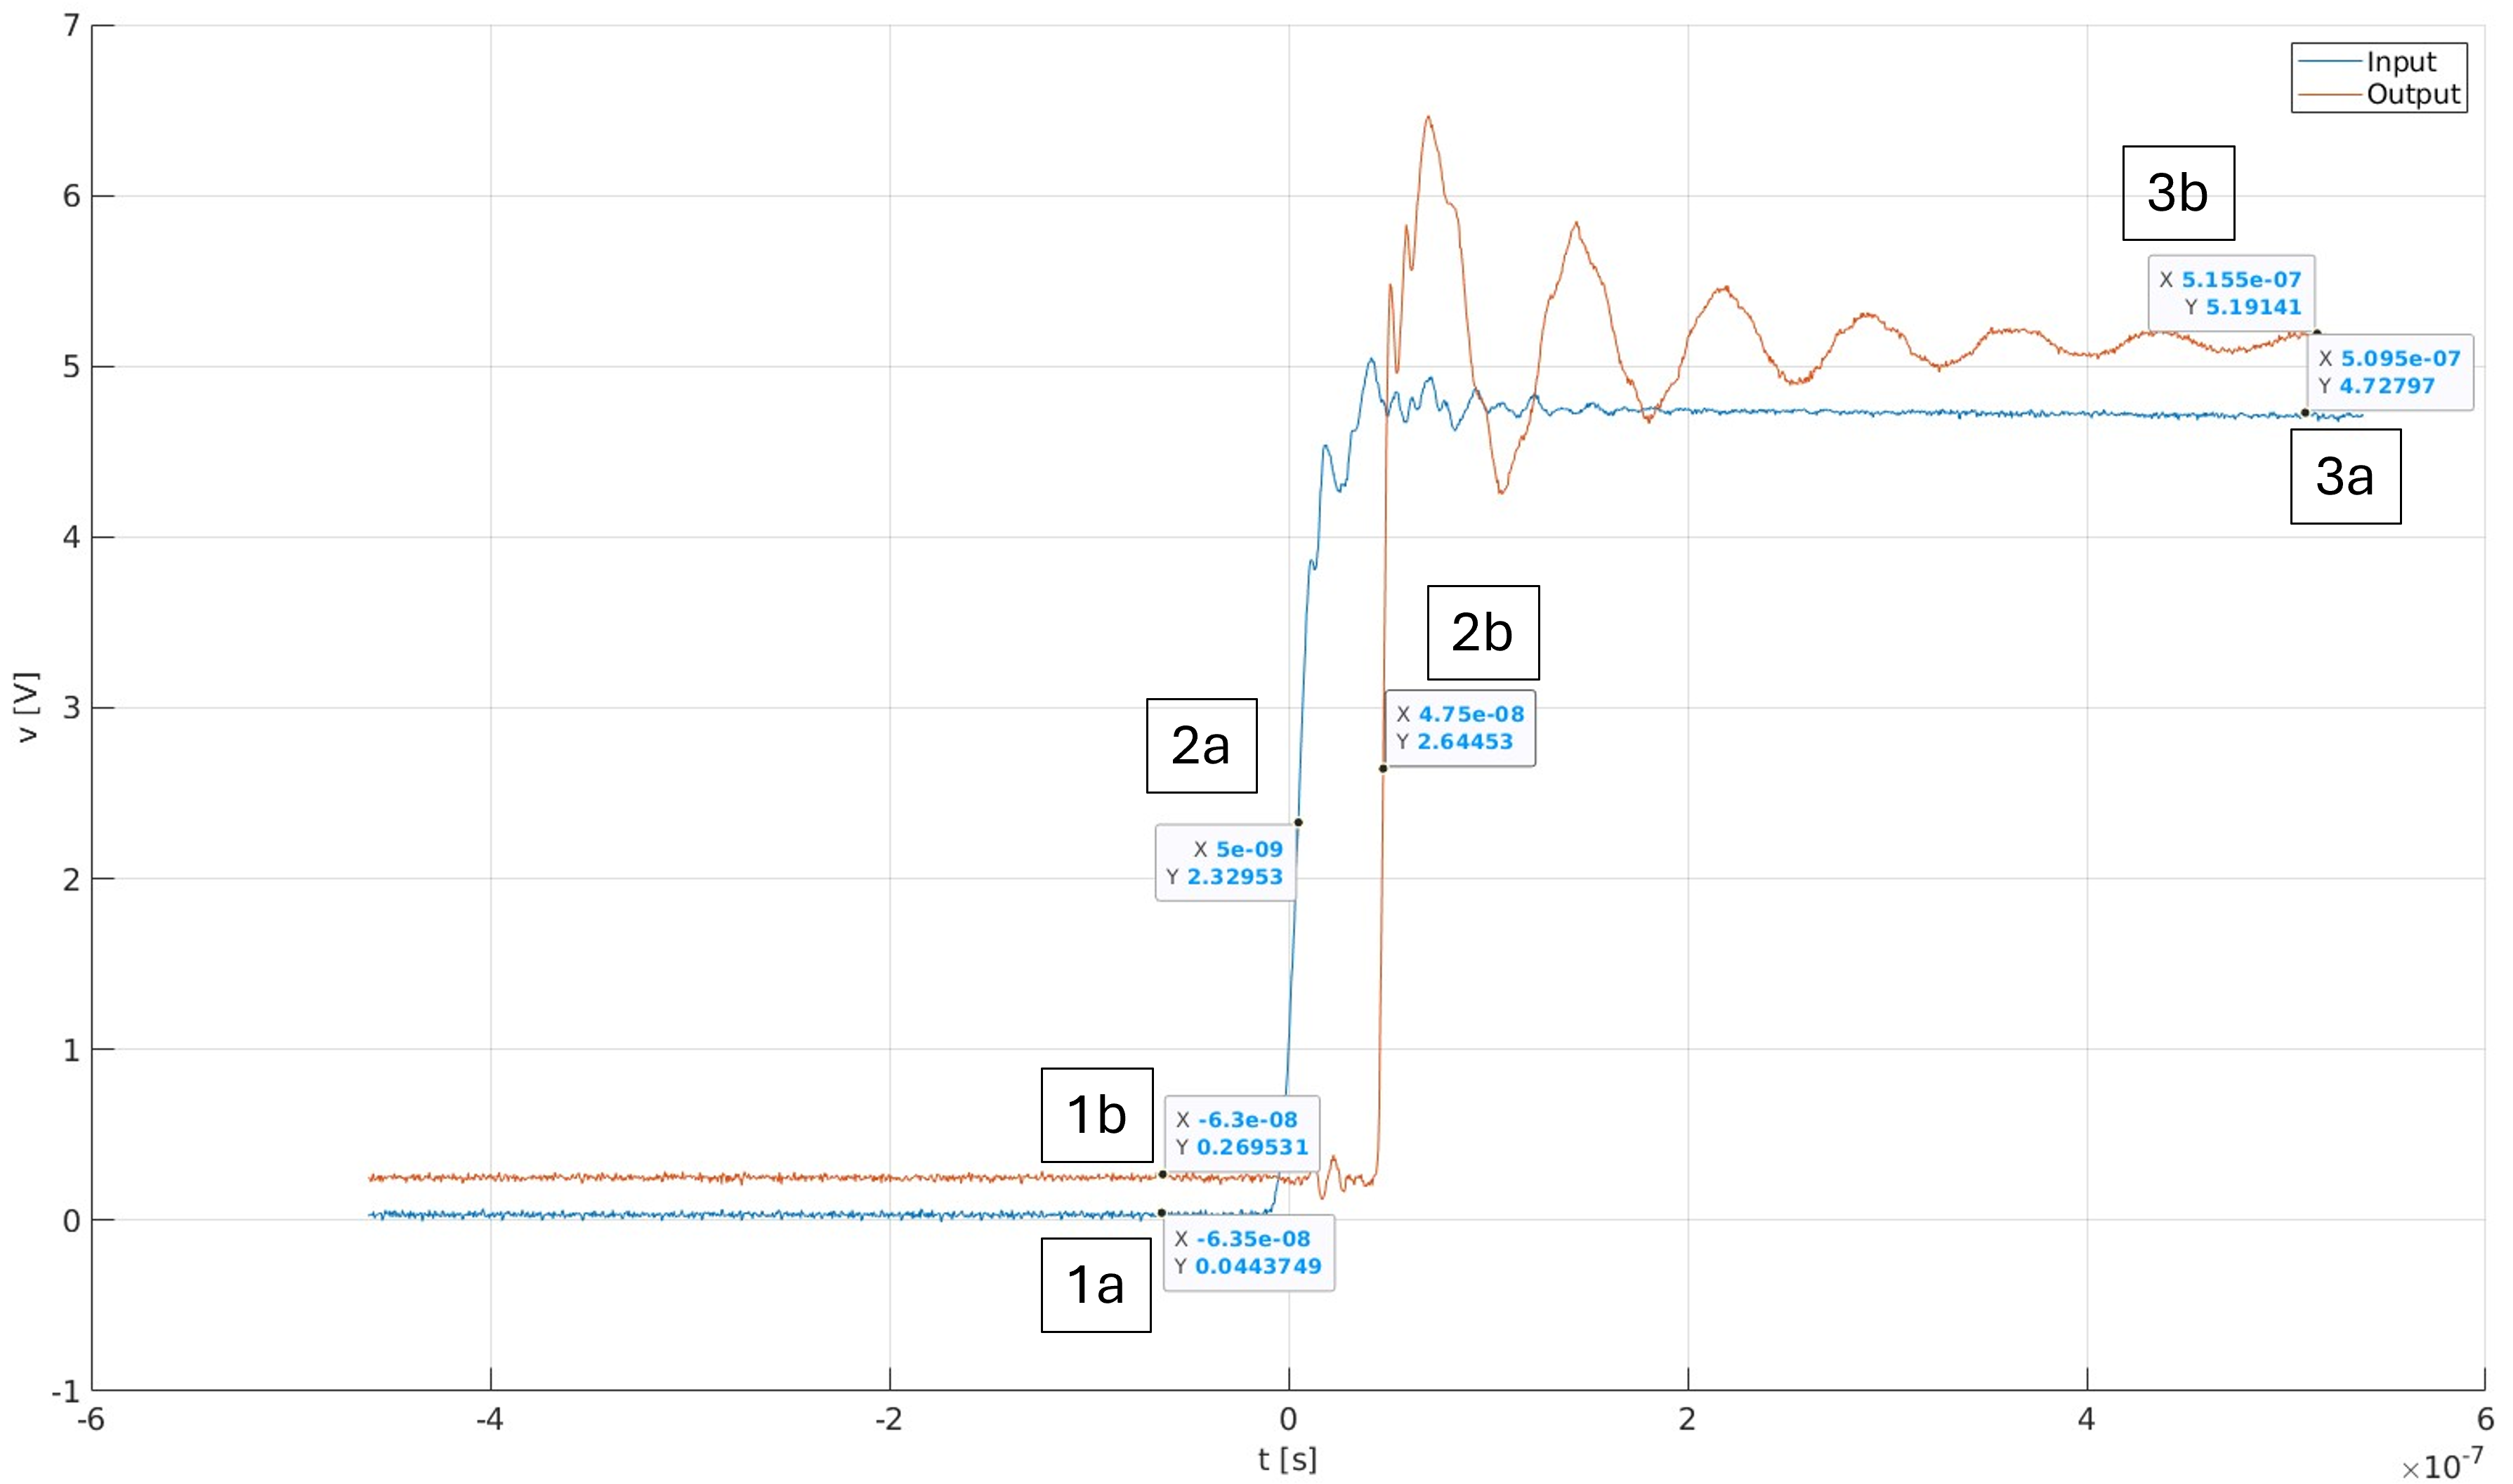
\includegraphics[width=0.75\textwidth]{4_inverters_marked.png}
    \caption{Rising edges of the input and output for the four inverter chain, with labeled marked points on the plot.}
    \label{fig:4inv}
\end{figure}

The same method for finding the total propagation delay is used for the four inverter-chain in figure \ref{fig:4inv} and is as follows:

\begin{align}
    t_{in} &= 5\mathrm{e}{-9} \ \text{s} \\
    t_{out} &= 4.75\mathrm{e}{-8} \ \text{s} \\
    t_{4inv} &= t_{out} - t_{in} = 4.45\mathrm{e}{-8} \  \text{s} \label{eq:4inv}
\end{align}

The values found in equation \ref{eq:3inv} and \ref{eq:4inv} are then used in equation \ref{eq:1inv} to calculate the propagation delay of a single inverter as follows:

\begin{equation}
    t_{1inv} = t_{4inv} - t_{3inv} = 1.55\mathrm{e}{-8} \ \text{s}
\end{equation}

\subsection{Discussion}
In the results section, both inverter chains are only plotted for either rising or falling edge. This is done on the assumption of equal time for both edges. This is not necessarily true, but the difference is assumed to be negligible.
 \paragraph*{}
The oscilloscope data depicted in Figures \ref{fig:3inv} and \ref{fig:4inv} suggests that the switching process is influenced by what appears to be an underdamped system response, where the measured signals at probes 2 and 3 exhibit oscillatory behavior prior to stabilizing. This oscillation introduces uncertainty in identifying the precise moment the signal reaches its high and low values, designated as points '1' and '3' respectively.
\paragraph*{}
This issue was mitigated by ajusting the reference points farther from the transition edges, allowing the transient response to decay. While this improves measurement stability and is more likely to yield consistency across multiple readings, it is essential to acknowledge that it does not guarantee absolute accuracy.

\paragraph*{}
The switching points were identified as the mid-level voltages between the high and low signal points, labeled as points '1' and '3' in Figures \ref{fig:3inv} and \ref{fig:4inv}. As such, the midpoints at which the signal transitions occur are designated as points '2a' and '2b.' It is important to note, however, that these identified switching points may not coincide precisely with the true thresholds of the logic levels due to the finite resolution of the oscilloscope. The samplerate of the measurement tool limits the ability to capture the exact moment at which the signal voltage crosses the threshold, introducing a potential source of error in the determination of the switching points.

\paragraph*{}
The implementation of an averaging filter played a crucial role in reducing noise within the output signal. This decision aimed to smoothen random signal variations, yielding a waveform that better represented the inherent characteristics of the inverter chain.
\paragraph*{}
Despite the filtering approach, it is acknowledged that the experiment was not conducted in a wholly controlled environment. Various stochastic variables could have affected the accuracy of the measurements, including but not limited to electromagnetic disturbances, fluctuations in the power supply, and thermal noise within the electronic components themselves. Recognizing these influences is vital for understanding the potential deviations in the reported results.

\end{document}